\subsection{Cache}
The cache will be utilized so that we do not have to make unnecessary requests to the connections when we are grabbing a user content on the respective service

\begin{figure}[h!]
	\centering
 	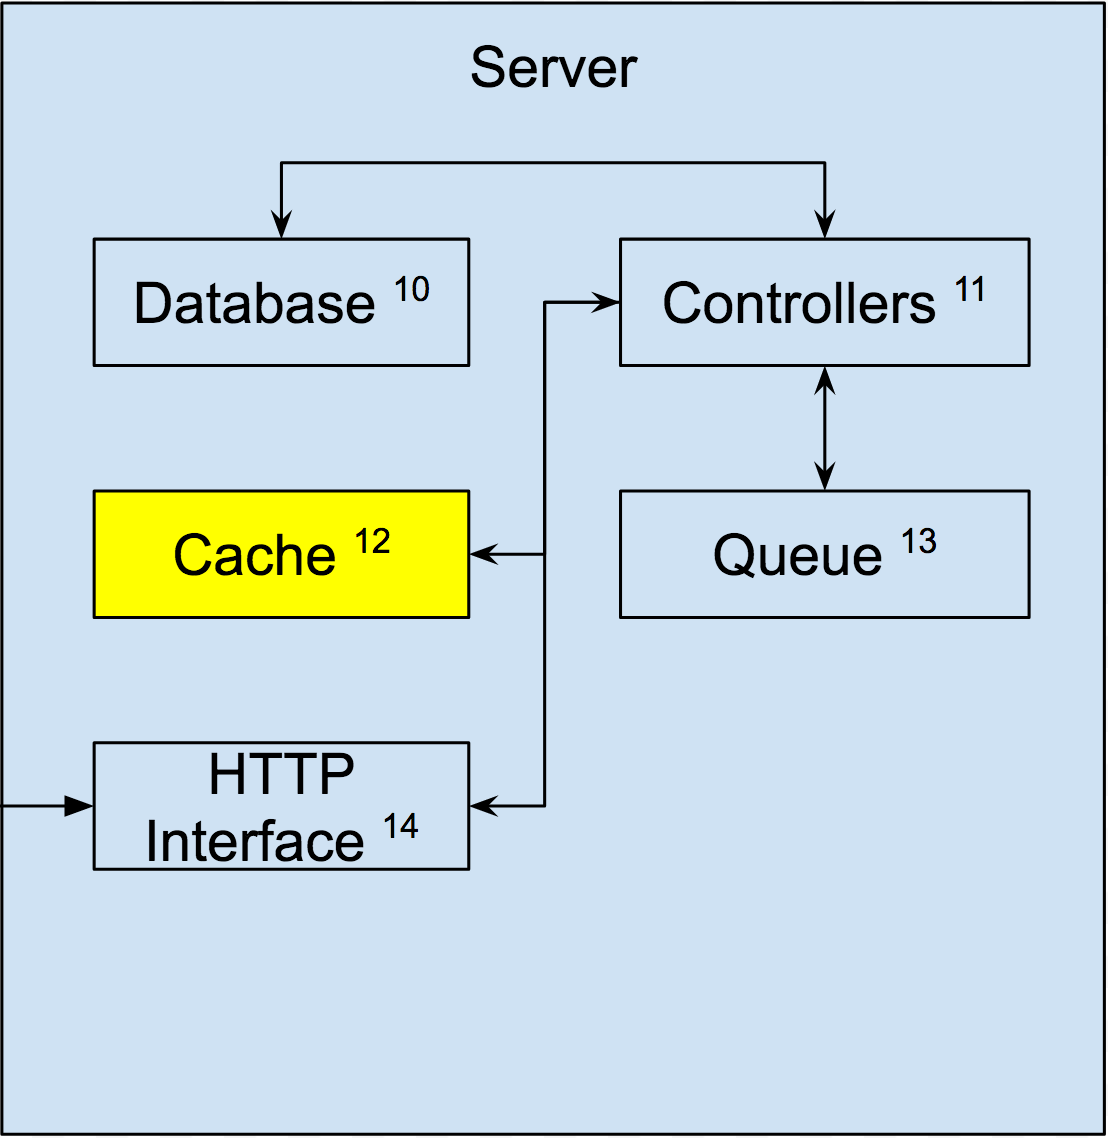
\includegraphics[width=0.60\textwidth]{images/server/server_cache.png}
 	\caption{Cache subsystem}
\end{figure}

\subsubsection{Subsystem Operating System}
N/A
\subsubsection{Subsystem Software Dependencies}
- Redis, "https://github.com/go-redis/redis" \\

\subsubsection{Subsystem Programming Languages}
Go
\subsubsection{Subsystem Data Structures}
Redis has many data structure built in that will provide us faster access to previously requested data, such as key-pair value maps with the option to expire, and weighted/sorted lists.
\subsubsection{Subsystem Data Processing}
In the event that our service via the Controller(s) goes out to one of the music services, we want to store that result in Redis in a key-pair value that will expire in 3-4 minutes later for later access.
\newpage
